\chapter{Webanalyse} %ca 8-10 Seiten
\label{ch:webanalyse} 

\section{Definitionen und Abgrenzung} % 1-1,5 Seiten
Die Webanalyse (engl. Web Analytics) ist ein Teilgebiet der Digitalanalyse (engl. Digital Analytics) und hat als Aufgabe, Webseiten zu analysieren und zu optimieren \parencite[Kap.1.2]{Hassler2019}. Die Abgrenzung zwischen Webanalyse und Digitalanalyse zeigt, dass sich die Webanalyse primär auf Daten bezieht, die aus dem Besuch und der Nutzung von Websites entstehen, wobei die Digitalanalyse den Rahmen erweitert und sich mit der kanalfübergreifenden Ermittlung von Nutzerbezogenen Daten beschäftigt \parencite[Kap.1.2]{Hassler2019}. Die Webanalyse wird von der Web Analytics Association (WAA) wie folgt definiert: \textit{``Web Analytics is the measurement, collection, analysis and reporting of Internet data for the purposes of understanding and optimizing Web usage.''} \parencite[3]{WAA2008}.

Eine weitere Definition liefert die ISO 19731:2017, welche Webanalyse als Analyse und Berichterstattung über das Verhalten, Aussagen und Stimmungen von Nutzern auf Online-Plattformen beschreibt \parencite[Kap.3.40]{ISO2017}. Diese Definition verdeutlicht noch einmal die Bedeutung von qualitativen und stimmungsbasierten Daten, welche auch bei der Analyse des Bildungsportals von Bedeutung sind.

Sie dient unter anderem dazu, die Herkunft von Nutzern, deren Klickverhalten sowie die Effektivität von Kampagnen und die Leistung einer Website zu analysieren. Erkenntnisse aus der Webanalyse unterstützen Unternehmen oder Organisationen dabei, ihre Inhalte entsprechend des Nutzerverhaltens zu personalisieren, Schwachstellen in der Nutzerreise auf der Plattform (engl. Customer Journey) zu identifizieren und die Nutzererfahrung (engl. User Experience) zu verbessern. \parencite{PiwikProWebanalyse}

\textcolor{red}{
    (wissenschaftlich sinnvoll/zielführend?, eigene Aussage:)Man könnte also sagen, die Webanalyse ist vergleichbar mit dem Beobachten und Dokumentieren des Verhaltens von Personen auf einem öffentlichen Platz. In beiden Szenarien wird erfasst, welche Wege die Besucher bevorzugen, welche Stellen eher gemieden werden oder auch wo sie am liebsten verweilen. Man kann beobachten woher die Leute kommen und auf welchem Weg.
}

Dabei ist jedoch zu berücksichtigen, dass die Webanalyse keine exakte Wissenschaft ist. Zum Beispiel unterliegen Daten zur Nutzeraktivität, wie Besucher- und Nutzungszahlen, unvermeidbaren Ungenauigkeiten, welche bereits bei der Erhebung und Verarbeitung entstehen können. Fragen nach der genauen Messung aller Besucher, der Unterscheidung von menschlichen und automatisierten Zugriffen sowie der Interpretation von Nutzungsverhalten verdeutlichen die Grenzen der Webanalyse. Dennoch liegt der Fokus nicht auf absoluter Präzision, sondern auf der Ableitung verwertbarer Trends und Veränderungen, etwa durch prozentuale Vergleiche. Dieser Ansatz ermöglicht es, relevante Erkenntnisse zu gewinnen, ohne dabei auf vollständige Genauigkeit angewiesen zu sein. \parencite[Kap.1.4]{Hassler2019}

Die Webanalyse basiert auf Metriken, beziehungsweise die Key Performance Indicators (KPIs). Sie ermöglichen es, die Interaktionen mit Websiten quantifizierbar zu machen, um datenbasierte Entscheidungen treffen zu können und Anhaltspunkte zu haben um das Nutzerverhalten einzuordnen. Im folgenden Kapitel werden die wichtigsten Metriken, sowie deren Bedeutung näher erläutert.

\section{Metriken, KPIs und Ziele} % 1-2
\label{sec:kpis}
Die von Herrn Staack beschriebenen Anforderungen werden im Folgenden spezifiziert. Hiebei sollen die Analysewerte so gewählt werden, dass sie zur Erfüllung der Anforderungen an die Nutzeranalyse beitragen. Zunächst ist es jedoch notwendig, die Begriffe \textbf{\glqq Metrik\grqq{}} und \textbf{\glqq Key Performance Indicator\grqq{}}, welche in Summe die Analysewerte darstellen zu definieren.

Eine \textbf{Metrik} ist eine messbare Größe, die eine bestimmte Eigenschaft beschreibt, ohne sie direkt zu bewerten. In der Webanalyse umfassen Metriken Werte wie Seitenaufrufe (engl. Pageviews), Besucherzahlen oder auch Besuche in Form von Sitzungen. Metriken helfen dabei, das Nutzerverhalten objektiv zu erfassen und die Leistung einer Website besser einzuschätzen. In der Webanalyse werden sie dafür eingesetzt, die online-Aktivität auf einer Website quantitativ zu messen. \parencite[Kap.5.1]{Hassler2019} \parencite[S.26]{Dykes2014}

Ein \textbf{Key Performance Indicator} wird oftmals mit einer Metrik gleichgesetzt. Allerdings handelt es sich hierbei um einen Teilbereich der Metriken. Eine KPI ensteht, wenn eine Messgröße mit einem konkreten Ziel verknüpft wird. Diese Zielbindung sorgt dafür, dass ein Indikator entsteht, welcher aufzeigt, wie gut oder schlecht ein Ziel erreicht wurde. Man kann also sagen, obwohl alle KPIs Metriken sind, sind nicht alle Metriken KPIs. \parencite[S.9-13]{Lammenett2019} \parencite[S.46]{Dykes2014}

Um die relevanten Metriken für das Bildungsportal \textit{evaschiffmann.de} zu identifizieren, wurden die spezifischen Gegebenheiten der Website sowie der Inhalt der Unterseiten berücksichtigt. Um das Nutzerverhalten detailiert zu erfassen wird darauf geachtet, dass die Analysewerte eine umfassende Analyse des Nutzerverhaltens ermöglichen. Somit wurde darauf geachtet Daten zu allen Kategorien einer Website zu erfassen. Der Autor Marco Hassler beschreibt in seinem Buch \glqq Digital und Web Analytics\grqq{} vier Kategorien oder auch Dimensionen einer Website, diese werden in Abbildung~\ref{fig:dimensionen} dargestellt \parencite[Kap.5.7]{Hassler2019}.: 

\begin{figure}[H]
    \centering
    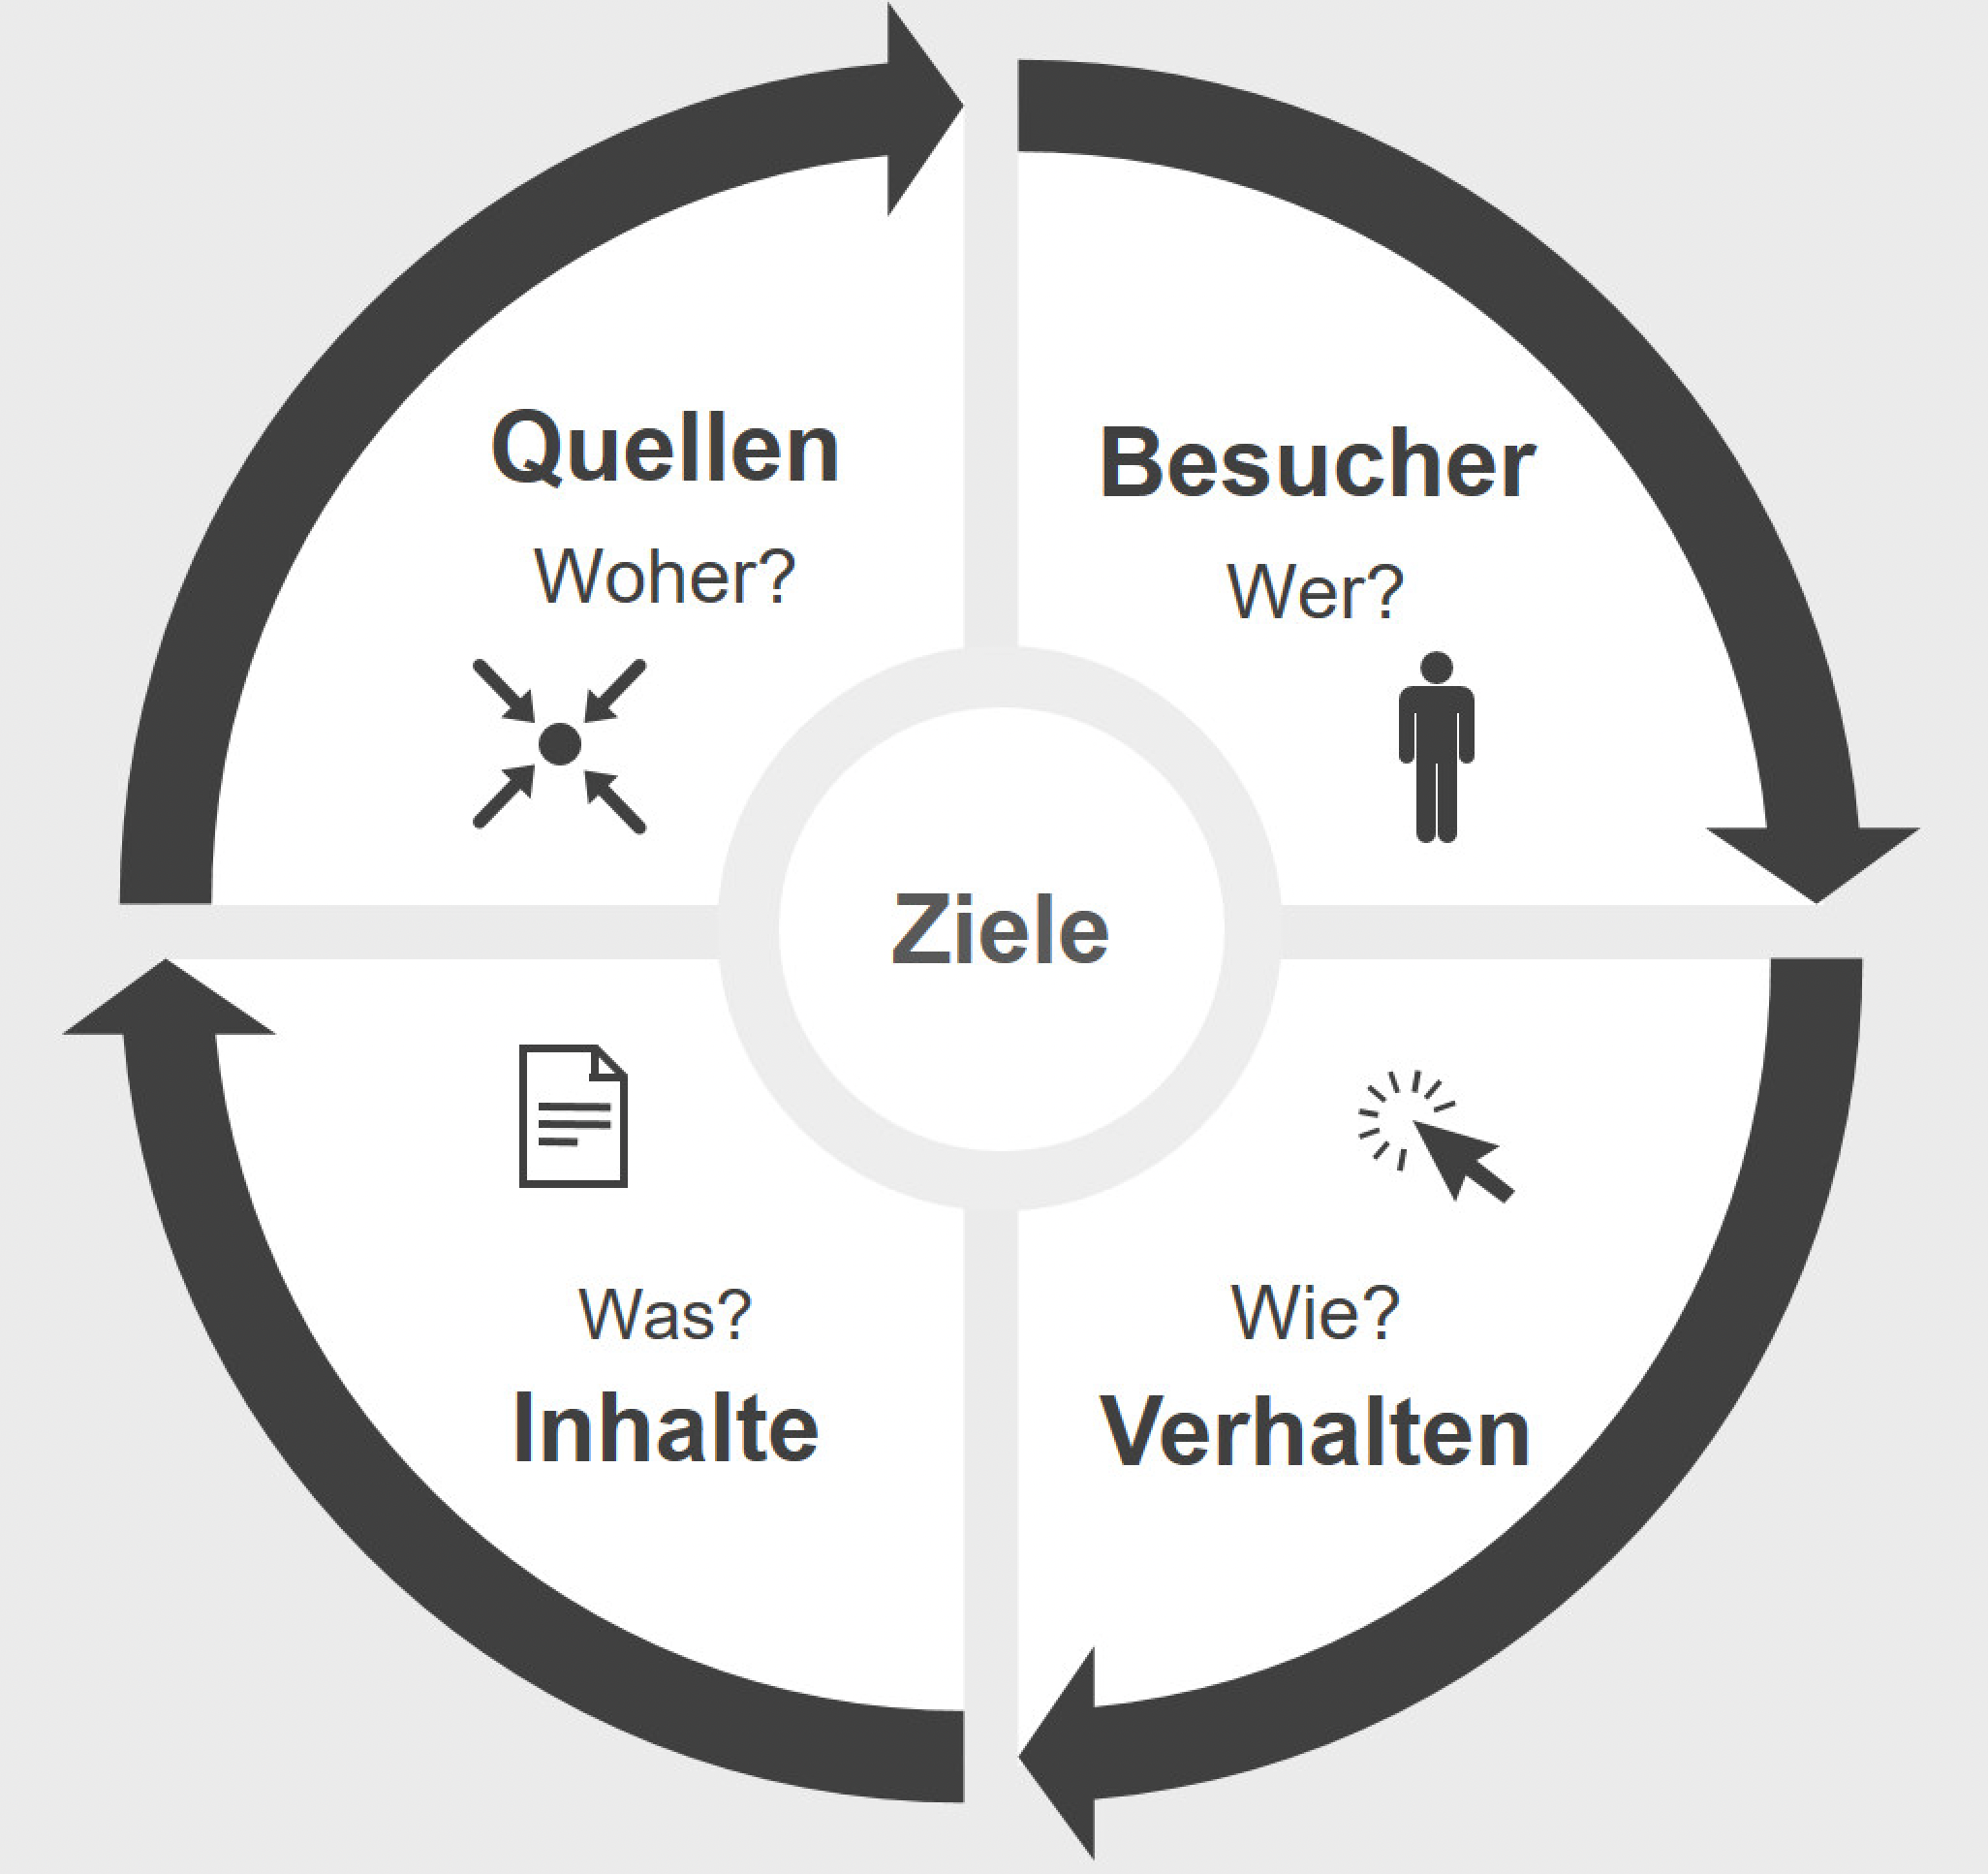
\includegraphics[width=6cm, height=5cm, keepaspectratio]{images/dimensionen.png}
    \caption{Metriken beleuchten hauptsächlich vier Dimensionen einer Website. \parencite[Kap.5.7]{Hassler2019}}%
    \label{fig:dimensionen}%
\end{figure}

Zusätzlich zu diesen Dimensionen beschreibt Hassler in seinem Buch \glqq Digital und Web Analytics\grqq{} die Wichtigkeit von Zielen bei der Webanalyse. Ziele sind essenziell, um den Erfolg der Website zu bewerten und sollten so gewählt werden, dass sie konkrete, messbare Nutzerinteraktionen widerspiegeln. Somit bieten Ziele einen Orientierungspunkt, um das Verhalten der Besucher besser einschätzen zu können. Um die Zielerreichung messbar zu machen kommen in der Webanalyse oftmals sogenannte Konvertierungen (engl. Conversions) zum Einsatz. Bei einer Conversion handelt es sich um eine Nutzerinteraktion, welche aus Sicht des Betreibers der Website als erwünschtes Verhalten gilt. \parencite[Kap.13]{Hassler2019}

Um diese Conversions in ein Verhältnis zu setzen, wird eine Konversionsrate (engl. Conversion-Rate) genutzt. Sie gibt das Verhältnis der Besucher einer Website zu den tatsächlich erfolgten Conversions an und wird in Prozent angegeben. Da bei einer Conversion-Rate Messgrößen mit einem konkreten Ziel verknüpft werden, spricht man hierbei von KPIs. \parencite{RyteConversion}

\textcolor{red}{
    (eigene Aussage basierend auf Erfahrungen/Recherche, Quelle notwendig?)Da es sich bei der Website \textit{evaschiffmann.de} nicht um eine E-Commerce Website handelt, sind die Ziele also unüberlicherweise keine kommerziellen. Trotzdem lassen sich Ziele definieren, welche einen Aufschluss darüber liefern, wie oft Besucher mit den Kernelementen der Website interagieren.
}

In der Tabelle~\ref{tab:analysewerte} werden alle Analysewerte, welche erfasst werden sollen mit der jeweiligen Dimension zu welcher sie zählen aufgelistet. In der letzten Spalte ist zu erkennen, ob es sich um eine Metrik oder eine KPI handelt. Zu beachten ist hierbei, dass sich manche Analysewerte aus mehreren Metriken zusammensetzen, wie genau diese Zusammensetzung erfolgt wird in der Sektion~\ref{sec:Visualisierungsmethoden} und dem Kapitel~\ref{ch:implementierung} ausführlich beschrieben.

\begin{table}[H]
    \centering
    \begin{tabularx}{\textwidth}{l l l}
        \hline
        \textbf{Analysewert} & \textbf{Dimension} & \textbf{Art der Daten} \\
        \hline
        Ranking der Referer Seiten & Quellen & Metrik \\
        Verteilung der Traffic Quellen & Quellen & Metrik \\
        Verteilung der Gerätetypen & Besucher & Metrik \\
        Anzahl der Besuche & Besucher & Metrik \\
        Anzahl der wiederkehrenden Besucher & Besucher & Metrik \\
        Anteil der wiederkehrenden Besucher & Besucher & Metrik \\
        Aufrufe der einzelnen Unterseiten & Inhalte & Metrik \\
        Ranking der am häufigsten aufgeklappten Überschriften & Inhalte & Metrik \\
        Verweildauer & Verhalten & Metrik \\
        Bounce Rate & Verhalten & Metrik \\
        Konversion: min. 1 Tagebucheintrag geöffnet & Ziel & KPI \\
        Konversion: min. 3 Tagebucheinträge geöffnet & Ziel & KPI \\
        Konversion: min. 1 Überschrift aufgeklappt & Ziel & KPI \\
        Konversion: min. 3 Überschriften aufgeklappt & Ziel & KPI \\
        \hline
    \end{tabularx}
    \caption{Analysewerte und ihre Klassifizierung nach Dimensionen}
    \label{tab:analysewerte}
\end{table}

\section{Datenerfassung}
\label{sec:Datenerfassung}
\subsection{Logfile-Analyse}
Die ersten Webanalyse-Tools basierten auf der Analyse von Logdateien (engl. Logfiles). Jedes Mal, wenn ein Nutzer eine Webseite aufruft, sendet sein Browser eine Anfrage an den Webserver, um die Inhalte der Seite zu laden. Der Webserver zeichnet jede dieser Anfragen, auch „Hit“ genannt, in einer Logdatei auf. \parencite[S.8]{Dykes2014}

Diese Logfiles werden in Form von Textdateien gespeichert und bieten eine strukturierte Übersicht über alle Interaktionen auf dem Server. Die Erstellung von Logfiles erfolgt automatisch, indem der Webserver Interaktionen zwischen Nutzer und Webseite aufzeichnet. Sobald ein Nutzer eine Webseite aufruft, sendet sein Browser mehrere Anforderungen (Requests) an den Server, um die verschiedenen Elemente der Seite wie Texte, Bilder oder Skripte zu laden. Der Server liefert daraufhin die angeforderten Inhalte zurück (Responses) und speichert diese Vorgänge zeitgleich in einer Logdatei. Diese Dateien, die in der Regel täglich neu generiert werden, dienen als Quelle für die Analyse von Zugriffen auf die Website. \parencite[Kap.2.2]{Hassler2019}

Im Listing~\ref{lst:logfile} ist ein Beispiel eines Logfile-Eintrags im Common Logfile Format (CLF) zu sehen:

\lstinputlisting[caption=Logfile-Eintrag im CLF \parencite{ApacheLogFiles}, label={lst:logfile}, language=Apache]{listings/logfile_entry.txt}

Aus diesem Beispiel eines Eintrags lassen sich folgende Informationen in entsprechender Reihenfolge entnehmen \parencite{ApacheLogFiles}: \\


\begin{itemize}
    \item IP-Adresse des Aufrufenden
    \item Identitätskennzeichen
    \item Authentifizierter Benutzername
    \item Aufrufdatum und Zeit
    \item URL der aufgerufenen Datei
    \item HTTP-Anfrage
    \item Ergebnis des Aufrufs (Status)
    \item Größe der zurückgegebenen Datei
\end{itemize}

Zusätzlich wird in der Logfile auch die Aufrufmethode (z. B. GET oder POST),  gespeichert, diese Angabe ist jedoch für eine spätere Analyse oft weniger relevant \parencite[Kap.2.2]{Hassler2019}. Der Vorteil dieser Methode ist es, dass die Datenerfassung unabhängig von Client-Technologien abläuft, da diese serverseitig erfolgt und keine zusätzlichen Technologien wie JavaScript notwendig sind \parencite{RyteLogFiles}. Der große Nachteil, wenn Nutzerdaten serverseitig erfasst werden ist es, dass clientseitige Informationen, welche nicht an den Webserver übertragen werden, nicht erfasst werden können. Somit werden Interaktionen mit der Website, welche keine Request auslösen nicht protokolliert und können nicht ausgewertet werden. Zudem können Seitenaufrufe (engl. Page Views), welche aus dem Browser-Cache geladen werden, nicht in den Logfiles erfasst werden. Ein Verfahren, welches für dieses Problem abhilfe schafft und Nutzer einer Website nicht aus der Sicht des Servers, sondern aus Sicht des Clients betrachtet, ist das sogenannte Page Tagging. \parencite{CounterCodePageTagging}, \parencite{CounterCodeLogFiles}

\subsection{Page Tagging}
\label{sec:pagetagging}
Unter Page Tagging versteht man die Einbindung eines kurzen Codeausschnittes (engl. Snippet) in den HTML-Code einer Webseite um Nutzerdaten zu erfassen. Dieses Snippet ist meistens in der Programmiersprache Javascript geschrieben. Das Snippet ermöglicht die Datenerfassung, indem es eine Javascript-Bibliothek herunterlädt, die im Cache-Speicher des Webbrowsers hinterlegt wird, um bei zukünftigen Seitenaufrufen schneller geladen zu werden. Nachdem das Page Tag die Bibliothek geladen hat, wird der Code ausgeführt, um verschiedene Daten aus dem Browser zu sammeln [Dykes, 2014, S.70-71]. Es können zum einen Daten abegerufen werden, welche per Browser Object Model (BOM) bezüglich der Einstellungen für den Webbrowser zu Verfügung stehen und zum anderen auch Informationen, welche das Document Object Model (DOM) enthält. Hierbei lassen sich unter anderem folgende Informationen per Page Tag sammeln [Hassler, 2019, Kap.2.3]:  

\begin{itemize}
    \item Mauszeigerposition
    \item Interaktionen mit Multimedia-Dateien
    \item Verweise in Form von Links
    \item Titel der Seite
    \item Tastatureingaben
    \item Bildschirmauflösung
    \item Cookies
    \item alle Informationen, welche auch Logfiles liefern
\end{itemize}

Um die gesammelten Daten an den Webserver zu übertragen, wird ein Bild in der Größe eines Pixels erzeugt, weshalb dieses Verfahren ebenfalls als Pixel-Tracking bezeichnet wird [Hassler, 2019, S.31]. Der Webbrowser erkennt dieses Bild als fehlenden Inhalt an, der geladen werden muss und sendet eine HTTP-Anfrage um es abzurufen. Diese Anfrage wird auch als Image-Request bezeichnet und enthält alle zuvor gesammelten Daten als Parameter in der URL. Die Image-Request wird allerdings nicht an den Webserver gesendet, auf welchem die Website hinterlegt ist, sondern an einen dedizierten Datensammlungsserver. Wurden die Daten vom Datensammlungsserver empfangen werden die Parameter aus der URL extrahiert und in einer Datenbank gespeichert. Anschließend können die Daten von einer Analyse-Engine verarbeitet werden um zusätzliche Einsichten in das Nutzerverhalten zu gewinnen. Neben der Verarbeitung der Daten kann der Datensammlungsserver in der HTTP-Antwort auch einen Cookie setzen. Dieser Cookie enthält eine eindeutige Kennung (Visitor-ID), die es ermöglicht, dass Gerät des Nutzers bei zukünftigen Besuchen wiederzuerkennen und gesammelte Daten mit diesem zu verknüpfen [Dykes, 2014, S.70-71].

- Grundlage von Page Tagging sind Events -> Überleitung

\subsection{Events}
Ein Event beschreibt eine gezielte Aktion, die auf einer Webseite durch einen Nutzer ausgelöst wird. Diese Aktionen werden entweder vom Browser oder vom Server protokolliert und mit einem Zeitstempel versehen. Events können unter anderem das Einblenden von Werbeanzeigen, das Beginnen oder Abschließen von Kaufprozessen, Änderungen in Formularfeldern oder das Abspielen von Videos sein. [WAA, 2007, S.33]

Für das Bildungsportal \textit{evaschiffmann.de} spielen Events somit eine essenzielle Rolle, wenn es um die Erfassung von Interaktionen mit Video- und Audioelementen geht. Ebenso werden Events unter anderem genutzt, um KPIs zu berechnen, welche sich auf die Nutzung der Suchfunktion, die Interaktionen mit der Karte oder das aufklappen von Überschriften beziehen. Events werden ebenfalls für die Aufzeichnung von Interaktionen mit eingebetteten Links verwendet [AT Internet, o.D]. Wie zum Beispiel das anklicken von Links, welche zu einem bestimmten Tagebucheintrag führen.

\subsection{Datenschutz und rechtliche Anforderungen}
\label{sec:datenschutz}
Die Analyse der Logfiles und besonders das Page Tagging, bieten umfangreiche Möglichkeiten zur Erfassung von Nutzerdaten. Im Umgang mit diesen personenbezogenen Daten muss allerdings einiges beachtet werden, um den gesetzlichen Datenschutzanforderungen gerecht zu werden. Im Folgenden werden die rechtlichen Aspekte und deren Auswirkungen auf die Webanalyse näher beleuchtet.

Der Datenschutz ist ein übergeordnetes Konzept, das in verschiedenen Ländern auf unterschiedliche Art und Weise geregelt ist. Die DSGVO hingegen stellt eine spezifische gesetzliche Regelung der EU dar, die alle Mitgliedstaaten gleichermaßen betrifft. Während Datenschutz allgemein darauf abzielt, die Privatsphäre der Menschen zu schützen, legt die DSGVO detaillierte Anforderungen an den Umgang mit personenbezogenen Daten fest und sieht hohe Bußgelder bei Verstoßen vor. Insbesondere für international tätige Unternehmen ist die Einhaltung der DSGVO essenziell, da sie auch außerhalb der EU gilt, wenn Daten von EU-Bürgern verarbeitet werden (Voigt \& Von dem Bussche, 2017, Kap.1; Kap.2).

Nach Art. 4 Abs. 1 DSGVO gelten alle Informationen, die sich auf eine identifizierte oder identifizierbare natürliche Person beziehen, als personenbezogene Daten (Europäische Union, 2016, Art. 4 Abs. 1). Hierzu zählen somit auch IP-Adressen und Cookies [Hanschke, 2020, Kap.2.4].

Art. 6 Abs. 1 DSGVO gibt vor, dass die Verarbeitung personenbezogener Daten nur rechtmäßig ist, wenn sie auf einer rechtlichen Grundlage beruht. Im Kontext der Webanalyse ist häufig die Einwilligung (Art. 6 Abs. 1 lit. a) relevant, welche vor der Datenerhebung eingeholt werden muss. Alternativ kann ein berechtigtes Interesse des Verantwortlichen (Art. 6 Abs. 1 lit. f) geltend gemacht werden, sofern die Interessen der Nutzer gewahrt bleiben (Europäische Union, 2016).

Die rechtlichen Anforderungen der DSGVO haben direkte Auswirkungen auf die Gestaltung und den Betrieb der Webanalyse. Als wichtige Aspekte gelten: 

\begin{itemize}
    \item \textbf{Transparenz:} Nutzer müssen darüber informiert werden, welche Daten erfasst werden und zu welchem Zweck [Hanschke, 2020, Kap.2.4].
    \item \textbf{Datenminimierung:} Analysesysteme sollten nur die für den jeweiligen Zweck erforderlichen Daten sammeln [Europäische Union, 2016, Art. 5 Abs. 1 lit. c].
    \item \textbf{Einwilligung:} Die Verarbeitung personenbezogener Daten geschieht oft durch den Einsatz von Cookies. Hierzu muss die Einwilligung der Nutzer eingeholt werden [Europäische Union, 2016, Art. 6 Abs. 1 lit. a]. 
    \item \textbf{?Rechenschaftspflicht?:} Unternehmen müssen nachweisen können, dass sie die Anforderungen der DSGVO einhalten. Dies erfordert technische und organisatorische Maßnahmen wie Dokumentation und Auditierung (Voigt Von dem Bussche, 2017).
\end{itemize}

Die IP-Adresse wird von der DSGVO als personenbezogenes Datum eingestuft, da sie in Kombination mit weiteren Informationen eine Identifizierung der Person ermöglichen kann. Analytics-Systeme müssen daher besondere Maßnahmen ergreifen, um die Verarbeitung der IP-Adressen DSGVO-konform zu gestalten. Häufig wird die IP-Adresse anonymisiert, bevor sie gespeichert oder weiterverarbeitet wird. Google Analytics beispielsweise bietet eine Funktion zur IP-Anonymisierung, bei der die letzten Stellen der IP-Adresse entfernt werden (Google, o.D.). % noch quellen suchen + PostHog

Cookies spielen eine zentrale Rolle in der Webanalyse, da sie es ermöglichen, Nutzer über verschiedene Sitzungen hinweg zu identifizieren. Die Verwendung von Cookies unterliegt jedoch strengen Anforderungen. Gemäß der E-Privacy-Richtlinie ("Cookie-Richtlinie") und der DSGVO ist für den Einsatz von Cookies, die nicht technisch notwendig sind, eine ausdrückliche Einwilligung der Nutzer erforderlich (Europäische Union, 2016). % Quelle + PostHog

Zusätzlich müssen Nutzer die Möglichkeit haben, ihre Einwilligung jederzeit zu widerrufen. Dies stellt hohe Anforderungen an die technische Umsetzung von Cookie-Bannern und Consent-Management-Plattformen (Trepte, 2021).

\section{Anforderungen an das Webanalyse-Tool} %3 Seiten
\label{sec:anforderungenWebanalyseTool}
Es gibt eine überwältigende Anzahl von Webanalyse-Tools, welche sich in ihren Funktionen, Kosten und technischen Ansätzen erheblich unterscheiden [Böhm \& Rittberger, 2016, S.244]. Grundsätzlich ist das Page Tagging besser geeignet, um detaillierte Informationen über das Nutzerverhalten auf Webseiten zu erfassen [vgl. Hassler, 2019, Kap.2.5.3]. Logfiles hingegen wurden ursprünglich zur technischen Überwachung entwickelt und enthalten nicht die hierfür erforderlichen Daten [vgl. Hassler, 2019, Kap.2.5.3]. Somit und mit den Erkenntnissen aus Kapitel~\ref{sec:pagetagging} wird deutlich, dass Page Tagging nicht nur umfangreiche Nutzerdaten liefert, sondern auch alle Informationen abdeckt, die durch die Analyse von Logfiles erfasst werden können. Weshalb bei der Auswahl einer Tool-Lösung ebenfalls darauf geachtet wird, dass die Daten per Page Tagging beziehungsweise per Events erhoben werden. 

Neben der Methode der Datenerhebung wurden noch weitere Anforderungen an das Webanalyse Tool definiert [vgl. Matomo, o.D.; CiteUp, 2024; Hassler, 2019, Kap.1.6]:

\begin{itemize}
    \item \textbf{Kosten:} Zunächst soll die kostenlose Variante eines Tools implementiert werden, um die grundlegenden Funktionen und die Eignung für das Bildungsportal zu testen, ohne dabei sofort finanzielle Mittel aufzuwenden.
    \item \textbf{Dokumentation:} Um die Implementierung zu erleichtern ist eine ausführliche Dokumentation für das Tool entscheidened.
    \item \textbf{Datengenauigkeit:} Es soll ein Tool ausgewählt werden, welches Datenaktualisierung in Echtzeit bietet um eine unverfälschte Basis für datengetriebene Entscheidungen zu gewährleisten. Ungenauigkeiten können sonst zu fehlerhaften Schlussfolgerungen führen.
    \item \textbf{Datenschutz und DSGVO-Konformität:} Wie in Kapitel~\ref{sec:datenschutz} erläutert, sind Datenschutz und die Einhaltung der DSGVO grundlegende Anforderungen an ein Webanalyse-Tool. Somit sollte dieses in der Lage sein, die geltenden Datenschutzgesätze einzuhalten.
\end{itemize}

\section{Matomo als Webanalyse-Tool}
Google Analytics (GA) ist mit einem Marktanteil von 82,0 \% unter den Websites, die Webanalyse-Tools verwenden, das mit Abstand am weitesten verbreitete Tool [W3Techs, 2025]. GA hat allerdings insbesondere in Europa stark an Akzeptanz verloren, da es wiederholt in Konflikt mit den Vorgaben der DSGVO geraten ist. Seit dem Ende des EU-US Privacy Shield ist die rechtliche Grundlage für die Übertragung von Nutzerdaten in die USA weggefallen, was dazu führte, dass Google Analytics mehrfach als nicht datenschutzkonform eingestuft wurde. [vgl. Förster, 2024]

Auf Grundlage dessen ist es keine Option GA für das Sammeln von Nutzerdaten auf dem Bildungsportal zu verwenden. 

Ein Tool welches eine datenschutzkonforme Erhebung der Nutzerdaten ermöglicht und ebenfalls selbst auf einem eigenen Server gehostet werden kann (engl. on-premise) ist Matomo [vgl. Förster, 2024]. Matomo sorgt dafür, dass Analysedaten auf einer Website gesammelt, gespeichert und in Form von Bereichten (engl. Reports) oder direkt über Anfragen an die Matomo Datenbank ausgeliefert werden können.
Das Tool ist Open-Source und kann auf verschiedenen Betriebsystemen wie Linux, Windows und macOS installiert werden. Alternativ dazu steht ebenfalls ein offizielles Docker-Image für die Bereitstellung in Container-Umgebungen zur Verfügung. Matomo benötigt eine MySQL oder MariaDB Datenbank um die Analysedaten zu speichern. 

Nachdem Matomo installiert und konfiguriert wurde, kann das Page Tag in den Quellcode der Website eingebunden werden, um die Erfassung und Übertragung von Nutzerdaten an den Matomo-Server (\texttt{matomo.php}) zu ermöglichen. Dabei wird der enthaltene Code bei jedem Seitenaufruf ausgeführt und sendet die gesammelten Daten an den Server. Das Page Tag verweist auf die Datei \texttt{matomo.js}, die als zentraler JavaScript Tracker fungiert und die eigentliche Tracking-Logik enthält. Nach der Datenerfassung sendet \texttt{matomo.js} die gesammelten Informationen in Form einer HTTP-Request an die Tracking-API \texttt{matomo.php} der Matomo-Instanz. Diese Instanz nimmt die Anfragen entgegen, verarbeitet diese und speichert die Rohdaten anschließend in der zugrunde liegenden Datenbank. Damit die Daten effizient abgerufen werden können, durchläuft Matomo einen Archivierungsprozess, bei dem die Rohdaten aggregiert und für die Erstellung von Reports optimiert werden. Diese Reports können über die Matomo Reporting API abgerufen werden. [Matomo, o.D.]

Matomo ermölgicht es außerdem eigenen Events zu definieren, um zum Beispiel Nutzerinteraktionen mit den ausklappbaren Überschriften oder das Abspielen von Videos auf dem Bildungsportal zu erfassen. Jedes Event besteht aus einer Kategorie und einer Aktion. Optional können Events ebenfalls noch einen Namen und einen Wert enthalten. Ein Beispiel für eine Funktion, welche ein solches Event triggert ist in Listing~\ref{lst:exampleEvent} zu sehen: 

\FloatBarrier
\lstinputlisting[caption=JavaScript-Funktion zur Erfassung eines Klick-Events auf einen Tagebucheintrag in Matomo, label={lst:exampleEvent}, language=java]{listings/exampleEvent.txt}

In diesem Beispiel wird ein Event erstellt, welches erfasst, wenn ein Nutzer einen Tagebucheintrag öffnet. Die Methode \texttt{\detokenize{_paq.push([])}} weist Matomo an, Daten in die Plattform zu übertragen, während \textbf{trackEvent} den Typ der gesendeten Daten definiert. Matomo erkennt die folgenden Parameter als Event-Attribute:

\begin{itemize}
    \item \textbf{DiaryEntry} ist die Kategorie, welche alle Ereignisse im Zusammenhang mit Tagebucheinträgen gruppiert.
    \item \textbf{DiaryEntryOpened} ist die Aktion, die angibt, dass der Eintrag geöffnet wurde.
    \item \textbf{DiaryEntryName} ist der Name, der den spezifischen Titel oder die ID des geöffneten Tagebucheintrags enthält.
\end{itemize}

Um nun das Event an der entsprechenden Stelle auszulösen, kann die Funktion innerhalb des entsprechenden HTML-Elementes eingebunden werden. Siehe Listing~\ref{lst:exampleEventCall}: 

\FloatBarrier
\begin{minipage}{\linewidth}
\lstinputlisting[caption=Event-Tracking für einen Klick auf einen Tagebucheintrag in Matomo, label={lst:exampleEventCall}, language=html]{listings/exampleEventCall.txt}
\end{minipage}

Hierbei wird das in Listing~\ref{lst:exampleEvent} definierte Event innerhalb des HTML-Elementes \texttt{<a>} ausgelöst und über das \texttt{onclick}-Attribut wird die Javascript-Funktion aufgerufen.

\textbf{Kosten} \\
Matomo kann neben einer kostenpflichtigen Cloud-Variante auch kostenlos auf eigenen Servern betrieben werden. 

\textbf{Dokumentation} \\
Matomo wurde bereits 2007 gegründet und war zunächst unter dem Namen Piwik bekannt [Matomo, o.D.]. Durch die langjährige Marktpräsenz hat sich eine umfassende Wissensbasis entwickelt, die sowohl eine offizielle Matomo Knowledge Base als auch eine Developer-Dokumentation umfasst. Ergänzt wird diese durch eine Vielzahl an praxisnahen Guides, Tutorials und Best-Practice-Beispielen. Somit bietet Matomo im Vergleich zu Tools wie PostHog, welches erst 2024 eine Webanalyse-Funktion eingeführt hat eine größere Wissensbasis, was die Einarbeitung in das Tool erheblich erleichtert. [vgl. Förster, 2024; Matomo, o.D]

\textbf{Datengenauigkeit} \\
->...kein Datasampling etc...

\textbf{Datenschutz und DSGVO-Konformität} \\
->vollkommen dsgvo-konform konfigurierbar, Cookieloses tracking möglich -> kein Cookie Banner notwendig